\documentclass[11pt]{report}

\usepackage{graphicx}
\usepackage{float}
\usepackage[parfill]{parskip}
\usepackage{rotating}
\usepackage{listings}
\usepackage{flafter} 
\usepackage{color}
\usepackage{cite}
\usepackage[round]{natbib}
\usepackage{comment}


\lstset{frame=tb,
  language=Python,
  aboveskip=3mm,
  belowskip=3mm,
  showstringspaces=false,
  columns=flexible,
  basicstyle={\small\ttfamily},
  numbers=none,
  breaklines=true,
  breakatwhitespace=true,
  tabsize=3
}
\usepackage{fancyhdr}
\setlength{\topmargin}{-.5in}
\setlength{\textheight}{9in}
\setlength{\oddsidemargin}{.125in}
\setlength{\textwidth}{6.25in}
\graphicspath{images/}
\begin{document}
\title{An Investigation into Network Emulation as a Testing Platform}
\author{Robert Game}
\date{}
\maketitle

\chapter*{Abstract}

In recent years technology for large enterprise has advanced significantly due to the introduction of virtualisation of infrastructure. This has allowed even the smallest of enterprise to adopt low-cost, virtual copies of their Production servers as a test bed and facilitates the segregation of Production and Development by holding a copy of the Production server for testing in Pre-Production. This means that when planning changes to a server it can first be tested in order to ensure that no unanticipated issues occur. This practise has been well adopted on the server infrastructure, however, when looking at network infrastructure there has not been significant uptake in the use of virtualisation to facilitate testing in this way. Many Network Operations teams rely on the use of a physical lab for the testing of changes, however these labs take considerable time to set up both from a cabling perspective and from configuring each device. This project aims to investigate more efficient methods of testing network changes through the use of router virtualisation. In order to do this I will investigate the Cisco's new product VIRL and how it can be used to create a tool which will provide a testing platform for network changes. In addition to simulating the network infrastructure this project will also investigate meaningful methods of creating testing evidence for use in large infrastructure. When implementing network changes in large infrastructure this is particularly useful evidence to have as Change Management teams continuously seek to avoid risk.

\pagebreak

\tableofcontents

\chapter{Introduction}

In recent years the use of a second, entirely separate infrastructure has been used to develop tools, test changes and simulate outages of IT Systems. In a large scale infrastructure these environments are usually created for testing changes on Server or Application environments, however the need for real traffic and the cost of dedicated hardware makes this difficult in the Network Infrastructure. The use of a physical lab takes time to set up and teams usually do not use them unless they are planning for large scale infrastructure changes.

This project will aim to create a tool intended for use in a Network Operations team in large scale enterprise. This tool will aim to pull together different aspects of Network Management tools and use information available to create a network model inside of the Cisco VIRL emulated environment. Using this model the Network Operations team can test environment changes on a model of their own network. Using data gathered from this simulation and the changes observed during any configuration edits the tool will then aim to create a piece of testing evidence which can be used to support any Change Management required on the infrastructure.

Large organisations, which are the primary target of the proposed tool, will often have Configuration Repositories and Configuration Management Databases (CMDB) that store relevant configurations and server locations. Alternatively, a networks team may want to generate a emulated version of an unknown network in order to understand its topology and configuration. The proposed tool will combine network emulation technology with these data sources to allow an Administrator to mimic changes to a production network and observe the impact that they have on data flow and connectivity. In particular the tool will generate testing evidence as proof of any impact (or lack of) when raising a network change.

The proposed tool provides value to a Network Engineer as it allows them to be more flexible in their network testing. With the proposed solution an Engineer will no longer need to create a physical clone of the network in a lab environment, nor will the need rely on outdated documentation. A emulated copy of the network can be produced from a node-edge representation of the topology along with the configurations for devices. This will save the Engineer time in the planning as well as allowing them to implement the changes in a non-production environment, in addition to the time savings an Engineer will also be able to produce testing evidence which can be used for Change Management purposes.

From initial findings it is understood that there are currently solutions for creating a simulated network, however, these tools rely on an Engineer to rebuild a network from scratch. Implementing the topology and interconnecting devices requires a well-documented network and in addition to the physical layout, the simulated devices also require a configuration which matches the real network. This project will aim to create a tool which will provide use to a Network Engineer regardless of the documentation they have for their infrastructure, allowing the Engineer to produce an emulated copy of their physical network without the need to reproduce the infrastructure on a device-by-device basis. The tool will produce an emulation of the network as a whole rather than focusing on devices.

\section{Scope}

This solution is targeted at medium to large enterprise which have a considerable routing set-up For example a global or regional backbone which connects multiple branch offices to a Headquarters. My tool will support both Interior and Exterior Routing protocols. In particular I am using my experience in the finance industry where Network Operations teams also work in an ISP role connecting through EBGP as well as traditional interior Distance Vector or Link State routing. This will create a tool that is scalable to the users needs, allowing a user to create a emulated copy of their local network through dynamic device discovery or a larger scale Engineer to produce an emulated version of a section of their network using Configuration Repositories and Network Diagrams.

\section{Objectives}
\begin{itemize}
\item{Create a tool which can take information from existing resources and create a working model of the Network Infrastructure within Cisco VIRL.}
\item{Extend the tool so that it can dynamically discover new network devices.}
\item{Facilitate the creation of a simulation within five minutes of starting the tool.}
\item{Produce a visual representation of the network for the user to view}
\item{Allow the user to interact with the emulation through traditional methods such as SSH or telnet}
\item{Investigate new methods for an Engineer to interact with a network}
\item{The production of detailed testing evidence during the simulation, such as neighbour tables, routing entries or link statuses.}
\end{itemize}

\chapter{Literature Review}

This chapter will review current publications in the field of network simulation and testing, I will use this literature first to gain inspiration for this project but also as a gap-analysis of the proposed tool. It will first focus on the use of Virtualisation in computer infrastructure, before looking at the use of network management techniques to gather information about a the infrastructure before finally focusing on 'What-if?' scenarios on a network and which tests are of most beneficial to a Network Engineer.


\section{Virtualisation of Infrastructure}

Virtualisation of infrastructure components has grown rapidly in the previous decade with the implementation of Cloud Computing being ``one of the most explosively expanding
technologies in the computing industry today'' \citep{younge2011analysis}.

The technology relies on creating a sandbox within a physical host in which ``multiple operating systems can safely coexist on one physical machine'' \citep{mergen2006virtualization} these virtual operating systems are governed by a tool known as a Hypervisor or Virtual Machine Monitor which ``safely multiplexes the hardware resources of the physical machine but leaves the specific hardware resource allocation to the operating system in the virtual machine'' \citep{mergen2006virtualization} creating the illusion to these virtual operating systems that they have full control of their hardware when in fact they are running in a sandbox environment cut-off from the 'real' hardware. 

The benefits of server virtualisation come in both a technical and economic form. \citep{crosby2006virtualization} says ``the artifacts of current operating-system and system-software architecture result in most servers today running at under 10 percent utilization.'' from a technical perspective the implementation of a virtual server for multiple operating system instances versus a separate physical host each allows for much better utilisation of a single server and thus provides gains in capacity management for infrastructure. Economic benefits come from the amount of physical hardware required in a Data Centre, \citep{daniels2009server} says ``Data center floor space and rack space are prime real estate in computing environments. Cooling and electricity costs have risen in recent years'' and the adoption of virtual infrastructure can help keep costs down which allows enterprises to implement practises such as High Availability services.

\begin{comment}
At first glance the adoption of virtual infrastructure may seem to only bring benefits to enterprise, however \citep{kotsovinos2010virtualization} highlights some issues that arise with implementing virtualisation technology in large infrastructure. In this article the author talks about issues such as System Sprawl where `developers forget to return the VMs they do not use to the pool after the end of a project' creating problems in accountability and server ownership. In addition to this there is also a breakdown in the conventional responsibility of teams (silos) as issues can arise from multiple areas of infrastructure, the author says `cross-silo collaboration and communication are of paramount importance, requiring a true mentality shift in the way enterprise infrastructure organizations operate' which may be difficult to implement. A third issue that arises is the added complexity of changes as `Sharing the infrastructure comes with centralization and, therefore, with potential bottlenecks that are not as well understood' this creates additional complexity in Change Management as it is no longer as clear how a decision can affect the infrastructure as a whole.
\end{comment}

From the literature it is clear that virtualisation is a technology which is gaining momentum in large enterprise. The use of which allows engineers to make use of their infrastructure efficiently in both capacity and cost. It is clear that virtualisation is the correct method of implementing a network testing tool due to it's scalability and ease of implementation when compared to physical equipment. 

\section{Virtualisation of Network Components}

From a testing perspective, virtualisation in the network infrastructure comes in the form of device emulation. \citep{galan2004use} discusses the use of virtualisation tools within a network lab, 
in this paper the author describes a scenario in which they have used a virtual network as a platform for learning. Features such as the ability to quickly create a simulation and the ease of restoring defaults when problems arise are highlighted as a significant benefit of simulation over real devices, particularly in a learning environment where misconfigurations are likely to occur. However, the author also highlights opportunities that are missed with simulated devices, such as having no physical contact with the routers means that hands-on experience is lost.

\citep{Knight:2012:ASL:2342356.2342378} says ``Emulated networks, which run a real router operating systems inside virtual machines, offer realistic yet inexpensive network experimentation. However they are time-consuming to configure, which limits their use in network research''. In this paper there is a proposal of a tool to simplify the creation of emulated networks, Autonetkit, which provides the ability to generate thousands of lines of configuration code across multiple devices from a high-level description of the topology as a whole. In particular this paper highlights the difficulty faced when creating an emulated network from scratch. When dealing with networks of hundreds or possibly thousands of nodes the time taken to configure each can outstrip the benefits of an emulated network.

This section of the Literature Review has given views on both the benefits and shortfalls of using virtualisation in network infrastructure. A significant benefit to network emulation is cost, with physical devices there is a significant investment in a single device with most requiring a support contract. For a large organisation this may be seen as an unnecessary expenditure, whereas the licensing cost for a VM may be considerably more cost effective. One shortfall of emulation that has been identified in the literature is the difficulty of defining a network from scratch, this will be taken into consideration when designing the proposed solution.

\section{Network Management and What-if? Scenarios}

Configuration and Change Management is a particularly important aspect in modern infrastructure systems, in particular improved vigilance on Change Management to Networks can improve reliability and uptime in for systems as a whole. \citep[p.270-273]{bellovin2009configuration} discusses these aspects both from a network and whole infrastructure perspective. In the paper's case study it talks of the importance of router configuration management to a large Internet Service Provider, one particular use of configuration management is understanding a malicious attack by viewing the current configuration as `the differences between the authorized configuration and the one installed by the intruder can give valuable clues as to goals and motives'

`What-if' scenarios are a section of Network Testing that allows an Engineer to understand how their topology will cope should an event occur. \citep{lad2006visualizing} discusses a potential solution to the uncertainty of a network change on the Internet, in this paper the author proposes a tool which allows the impact of a BGP update to be understood by providing a visual representation of changes to an Autonomous System's forwarding path. This tool allows an Engineer to understand where traffic is flowing in the event of a change to a network. However, this tool falls short as it only allows an Engineer to view routing changes in real-time instead of gaining an understanding of what could happen.

This section of the Literature Review was particularly difficult as there are very few tools available that allow both emulation of a real network and feedback on changes to the emulated network. This indicates a gap in current solutions which the proposed solution may be able to target.

\chapter{Current Solutions and Cisco VIRL}

\section{Current Solutions}

\subsection{Hardware}

Traditional approaches to Network Testing would rely on hardware to be a `true' copy of the Production Network. However as infrastructure grows and becomes more complex, the flexibility of this method diminishes. The use of hardware for testing relies on an organisation having a complete network lab on-site which an Engineer can use to build smaller sections of the Production network, replicating the topology by using identical device models to the production counterpart along with the same software version and running configuration. This creates an additional burden on any proposed changes to a Production network as every change requires a physical build of a clone of the network before testing can occur. In addition to the time cost associated with this testing, there is an additional monetary cost to an organisation as they need to hold additional hardware, usually with a large support contract attached, in order to be able to carry out testing. For some smaller enterprise this additional cost may not be viable and some risks may be taken by implementing changes without prior testing.

\subsection{Simulation}

Network Simulation extends the concept of testing by allowing a user to create a simulated network, however, this is not full emulation and is not as reliable as a testing tool when compared to other methods. In recent years simulation of networks has been used as a tool for vendor-specific educational courses such as Cisco's CCNA or Juniper's JNCIA certification programs.

Cisco's offering on the simulation market is an educational tool for basic learning of the Cisco Certified Network Associate (CCNA) certification. Packet Tracer \citep{ciscoPacketTracer} takes form as a topology view which allows a user to drag and drop routers and switches onto the topology. The devices run a simplified version of the Cisco IOS and allow the user to connect to the devices serial port in order to configure them. An example of Packet Tracer is shown in Figure 3.1.

\begin{figure}[h!]
	\caption{Cisco Packet Tracer}
	\centering
	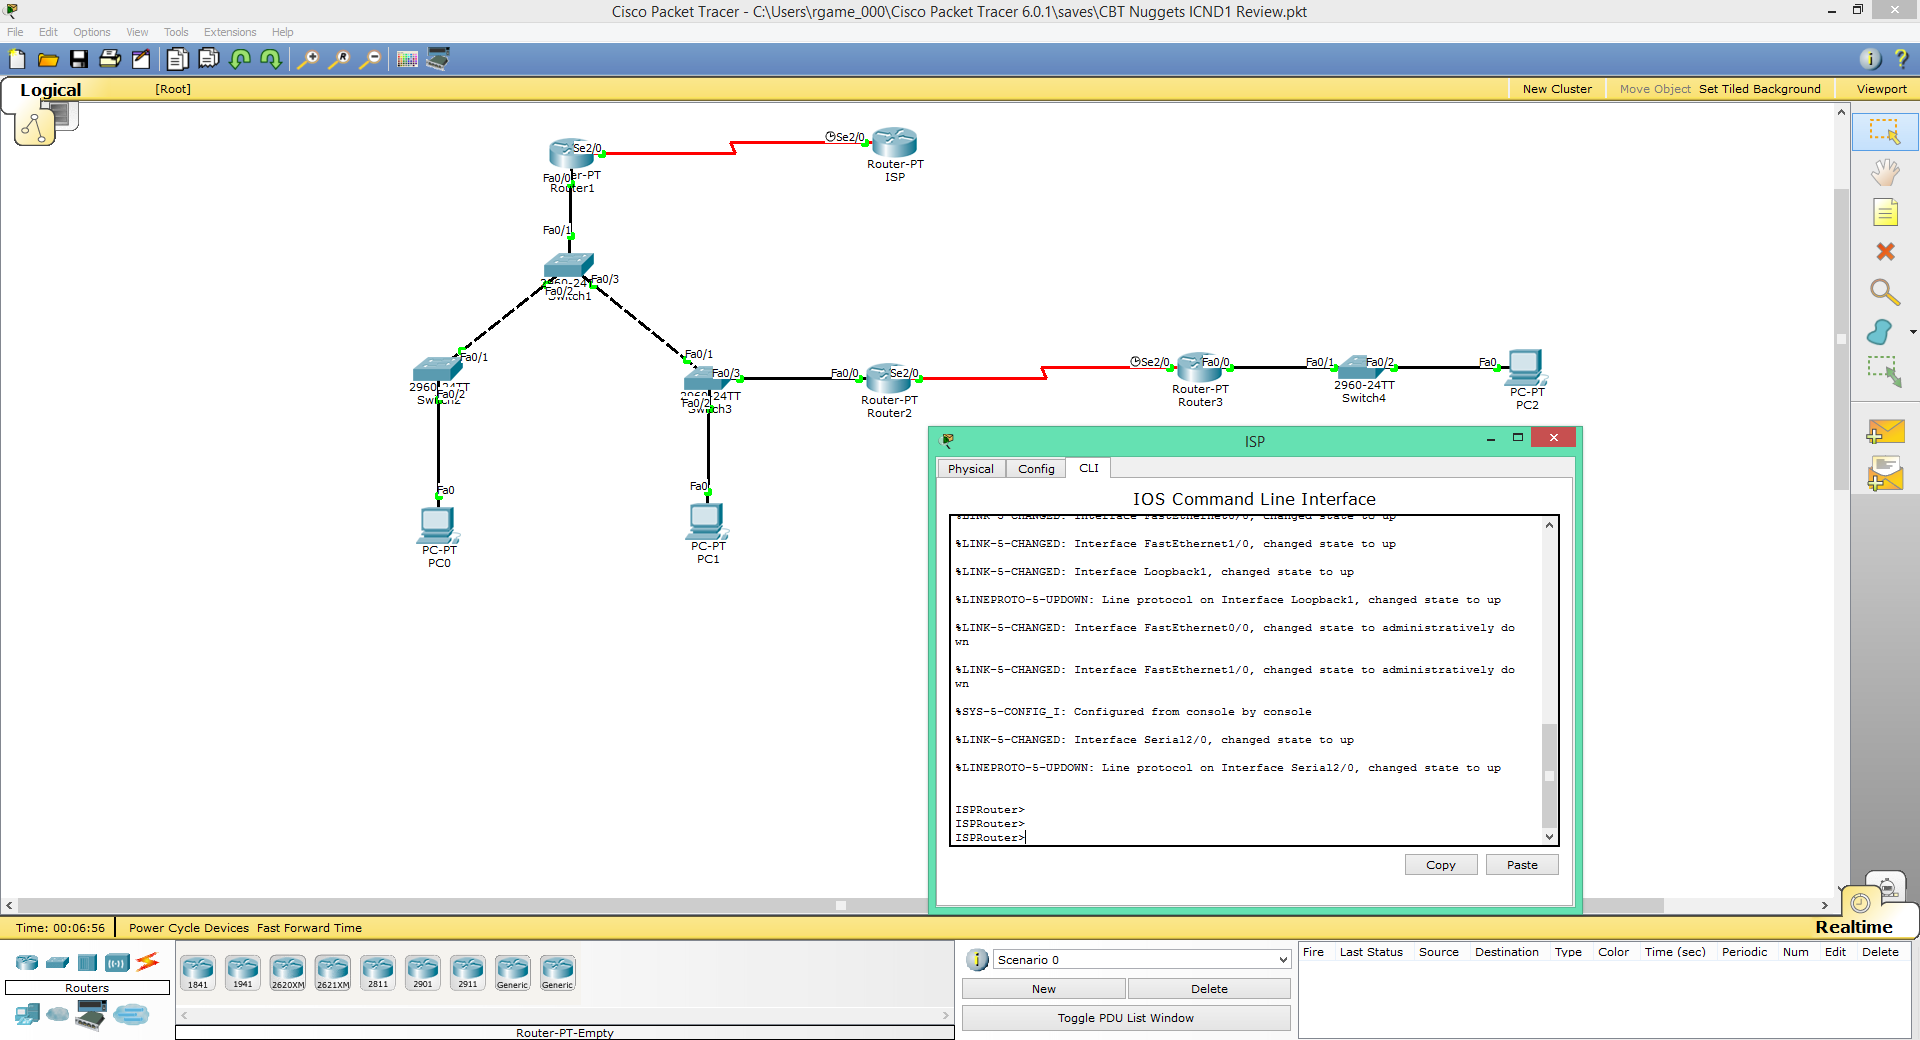
\includegraphics[width=1\textwidth]{packetTracer.png}
\end{figure}

 These simulations tend to focus on creating a learning environment for their tools and as such do not perform adequately as simulated `real world' devices. These devices tend to work as a simulator in that they mimic the behaviour of a network, and not the devices. For example, the software will decide to build an OSPF neighbouring should the required fields match on the devices. In contrast, a simulator (and real device) will build the relationship through a series of negotiations and packet transfers. As a result these simulators cannot be used reliably as network testing tool as the behaviour is predefined and may not be a true reflection of real hardware.
 
 Other network device vendors such as Juniper, HP and Huawei have offered simulated versions of their network equipment which work on similar principals, however these tools have not been a focus of this section as they do not emulate Cisco software.

\subsection{Emulation}

The Open Source community has also played a role in this virtual networks field, a project named GNS3 \citep{GNS31.2} was started in 2006 which aimed to create  unified tool to pull together hardware simulation and topology design into one UI. From this they created GNS3, a front end which allowed users to create a topology in a ‘drag and drop’ style and then start equipment as required. GNS3 is intended to be a multi-vendor tool but is particularly used for Cisco simulations. Using a hypervisor called Dynamips the tool can create a VM of a Cisco router which can be interconnected to create a real topology. In addition to this, GNS3 can be adapted as a network emulator, which enables a user to connect their simulated topology to their physical network.

\begin{figure}[h!]
	\caption{GNS3 1.2}
	\centering
	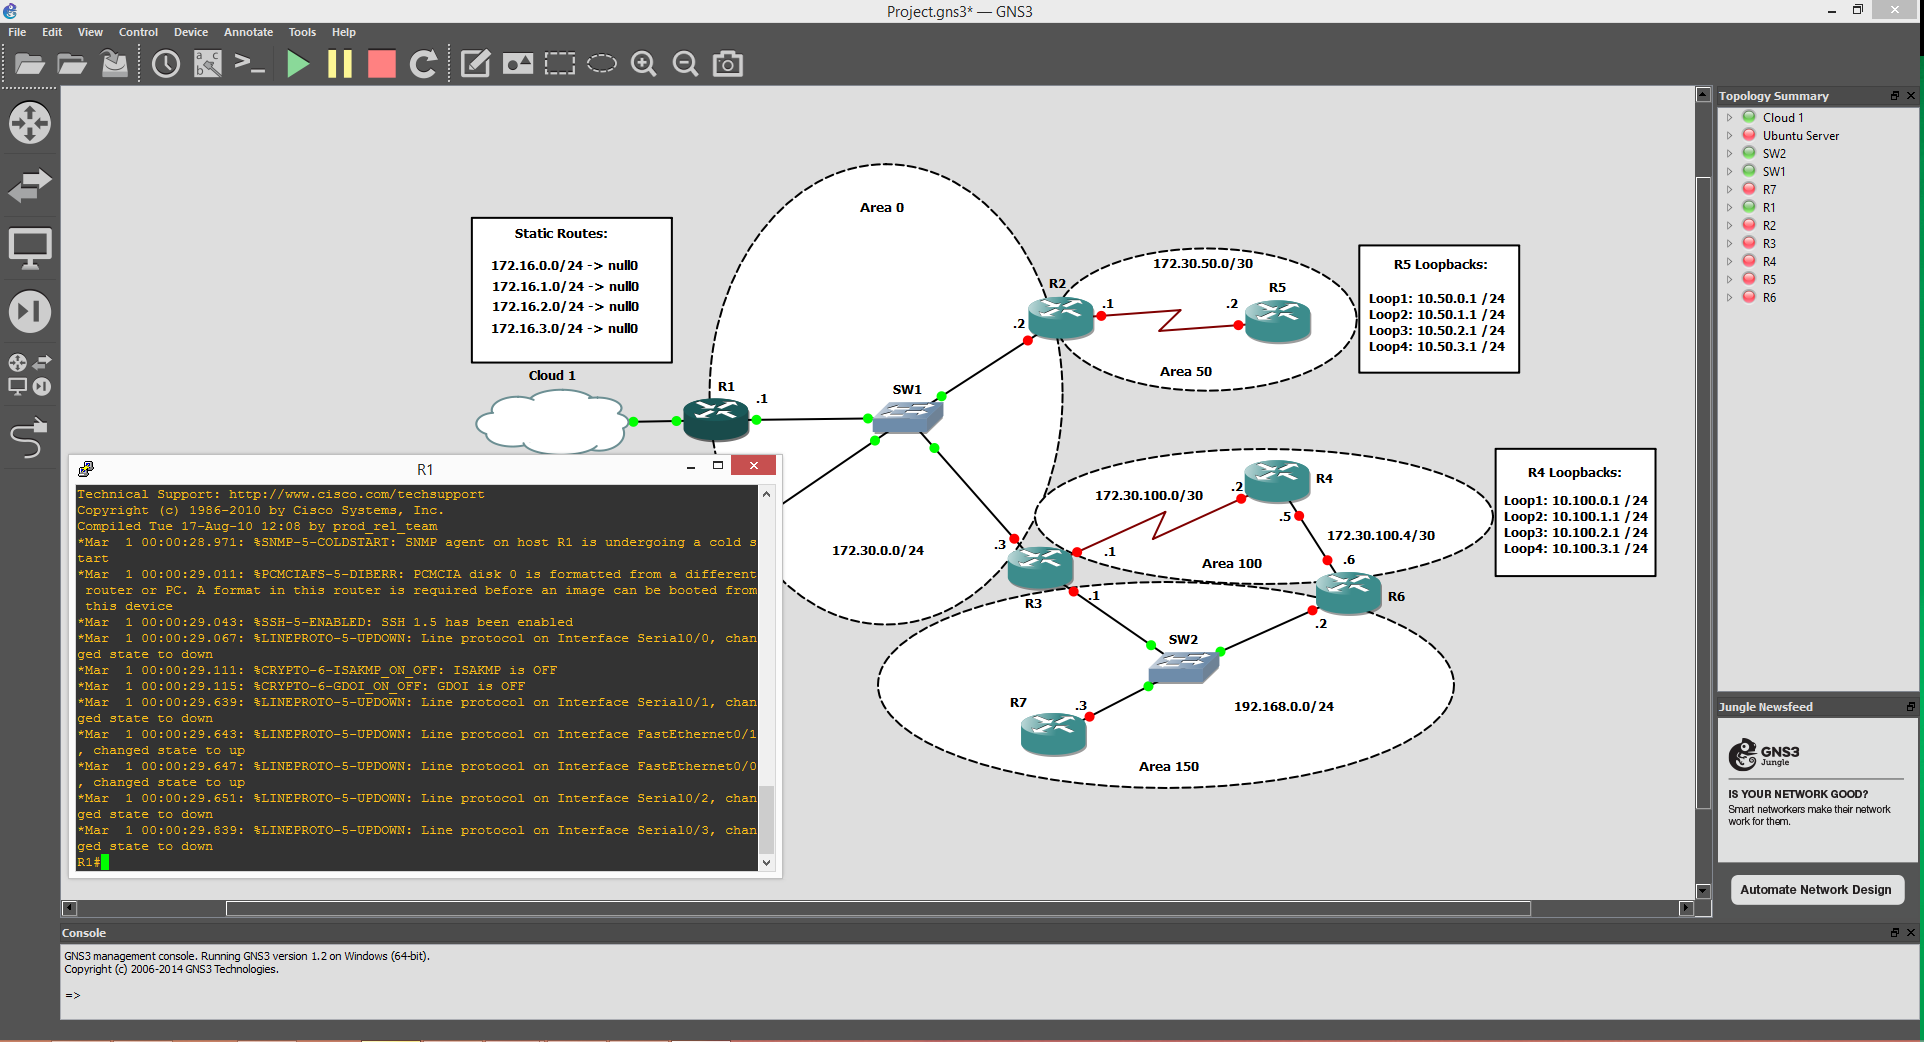
\includegraphics[width=1\textwidth]{GNS3.png}
\end{figure}

GNS3 works well for Cisco router simulation, however it falls short when looking at Layer 2 simulation. Features such as Spanning Tree Protocol rely heavily on the fast processing speed of Application Specific Integrated Circuitry (ASICs) which are controllers within the switches that can quickly process frames. Cisco IOS combined with Dynamips cannot process frames fast enough in order to successfully implement these protocols. Therefore when testing redundancy scenarios such as outages which force a Layer 2 topology change cannot be tested. In addition to the issues outlined above there is no support for network discovery and the building of topologies for network testing.

In addition to the shortfalls in some protocols, GNS3 lacks the scalability of some of it's competitors. On a conventional PC it can emulated 10-15 devices, however may use up to 90\% of the host's CPU if the IOS version is not calibrated for the host PC, because of this lack in scalability it may not be of any use to large enterprise.

From the review of current solutions there has not been a tool which can generate simulations of existing hardware. The only solutions at current are bare-bones building tool for network designs. The proposed tool is different in that its purpose is to be used in existing infrastructure to test disaster recovery or planned configuration changes.

\section{Cisco Virtual Internet Routing Lab (VIRL)}

Cisco VIRL is a relatively new offering on the Virtualisation market, VIRL is pre-release software which forms the back end for a future Cisco product called Cisco Modelling Labs. This tool provides emulation using a new version of Cisco’s IOS and NexusOS, tailor made for virtualisation and fast deployment.

VIRL is a relatively new offering from Cisco, and is their first software specifically created to support virtual copies of their routers. It was first released to the public in November 2014 as a stand-alone client installed on a local machine. However for the purposes of this Project I have been fortunate enough to have access to the University's own server-based version of VIRL. This provides support for up to 200 instances in comparison to the Personal Edition which is capped at 15 instances. This has enabled me to take advantage of extra features such as Servers which can be attached to a network topology, providing added features such as network analysis and traffic creation.

\begin{figure}[h!]
	\caption{Cisco VM  Maestro}
	\centering
	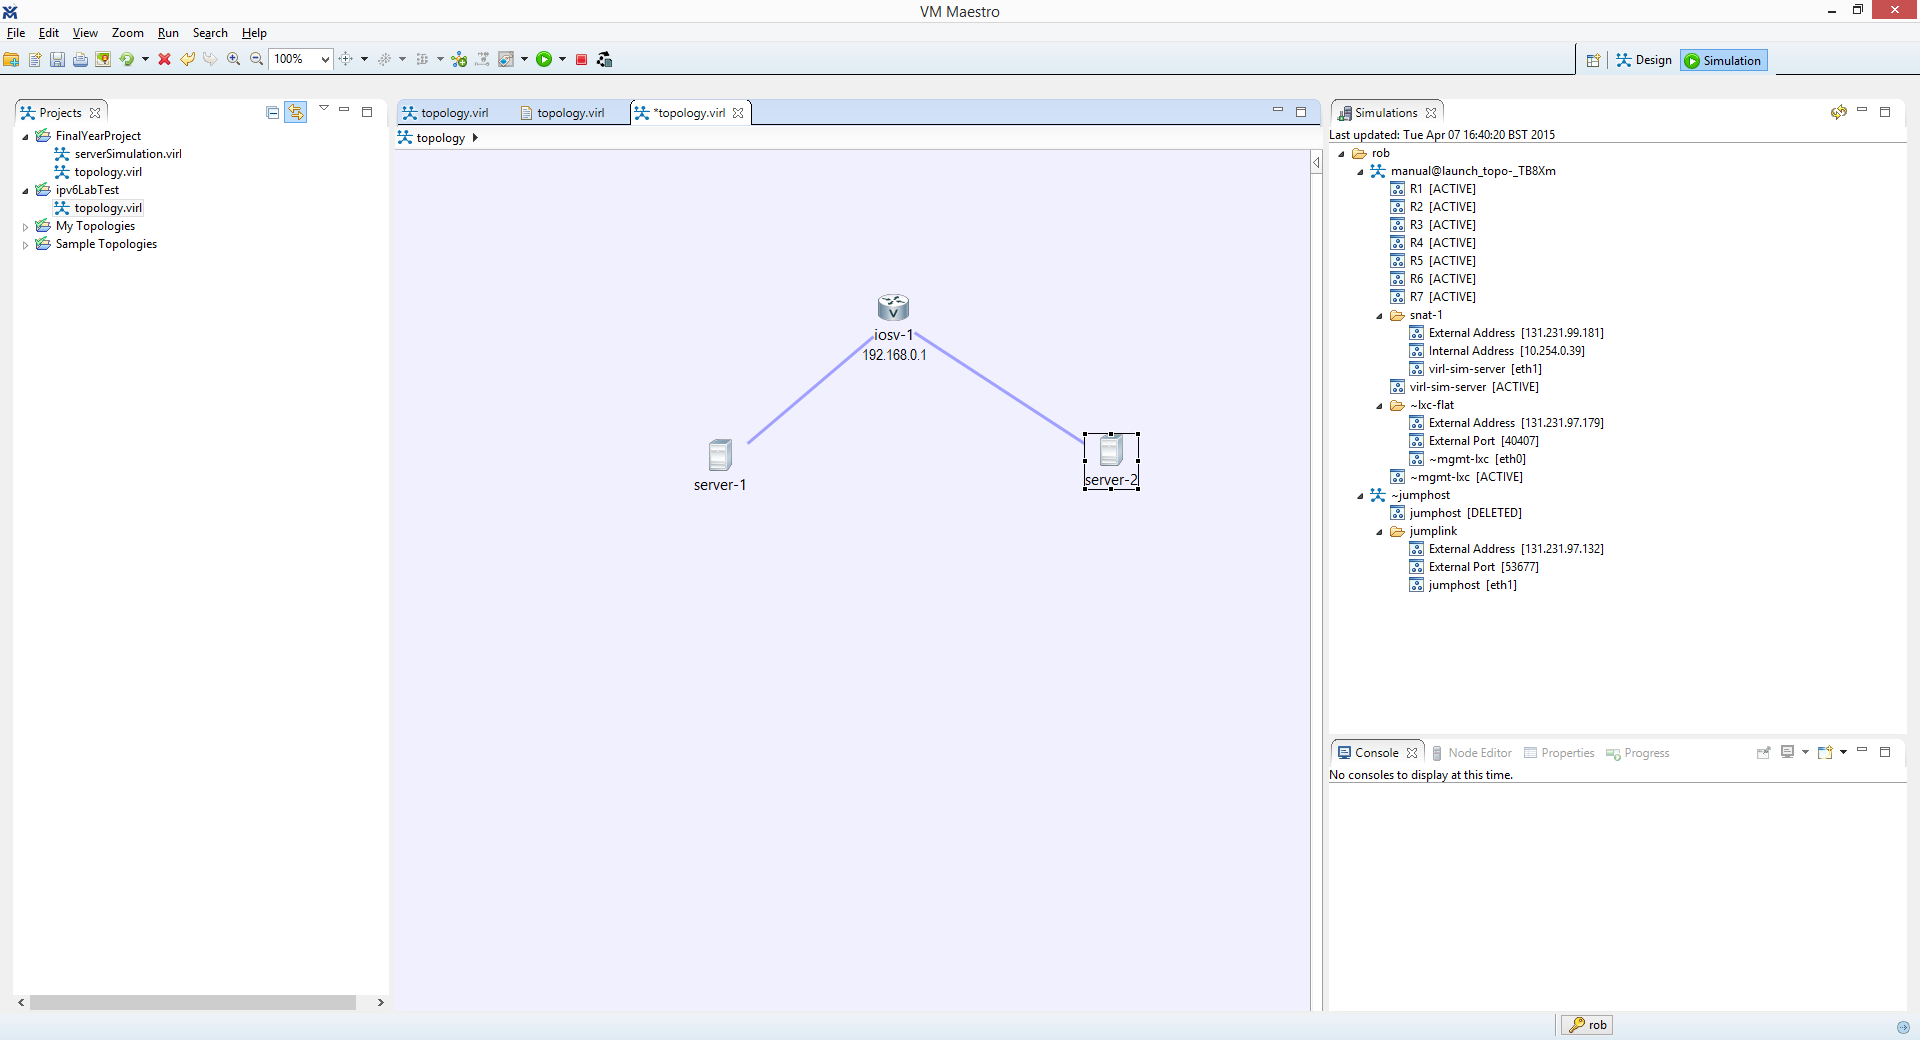
\includegraphics[width=1\textwidth]{VIRL.png}
\end{figure}

Connection to the VIRL Server is provided though an Eclipse-based front-end called VM Maestro. This interface provides an sandbox to build network topologies using the provided images of Cisco hardware within VIRL. For this project I will be concentrating on the use of Cisco's IOSv image, an image of the traditional IOS but adapted for use with a hypervisor. This allows the image to be run on a server without any dedicated ASICs. VIRL can then interconnect these devices provide connectivity and traffic. Using these connections the Routers can use routing protocols such as OSPF, EIGRP or BGP in order to create routing tables - this enables the user to simulate the Layer 3 functionality of their topology.

VIRL has also been designed with flexibility in mind for it's users, one specific feature of note is the support of a tool called Autonetkit. This integration allows VIRL to create a fully functioning topology in a matter of seconds as configurations such as ip addressing and routing protocols can be passed off to Autonetkit which will auto-generate a working topology.

In addition to the features provided for functionality within VM Maestro, there are also a variety of configurations available to connect VIRL to the outside world. The first available connection is FLAT Networking - this provides a layer 2 interface which can bridge VIRL with physical hardware. This is particularly useful as it allows a user to integrate Layer 2 functionality with their simulation, an area in which VIRL is currently lacking. The second method of connectivity is through a SNAT connection on the VIRL simulation, this allows the simulation to assign external addresses to simulated objects such as Routers and Servers.

Server support within VIRL is provided through pre-defined image varying in system requirements. The default images are Ubuntu but other images can be imported if required. These servers can be connected to the internet in order to customise them for to the users needs, an example would be installing an SNMP Server in order to poll the routers for information.

\chapter{Proposed Tool}

\section{High-Level Design}

At the highest level the proposed tool will provide an Engineer with an emulated version of their physical network for use as a test bed for changes or disaster recovery simulations. At a more granular level the tool is split into four distinct sections: Network Discovery, Network Representation, Emulation and Network Interaction. This chapter will focus on these sections from a design perspective, investigating how they can be implemented and which technologies can support their creation. Figure 4.1 shows these sections further broken down into separate sub-tasks.

\begin{figure}[h!]
	\caption{Step-wise Work Breakdown}
	\centering
	\includegraphics[width=1\textwidth]{work-Breakdown.png}
\end{figure}

The tool will be of a linear format, current expectations will be that the tool will generate a simulation from given inputs, at which point the user will be able to interact with the simulation and feedback of their changes will be available. Due to this linearity, the tool's functionality is best shown as the activity diagram in Figure 4.2 

\begin{sidewaysfigure}[h]
	\caption{Activity Diagram}
	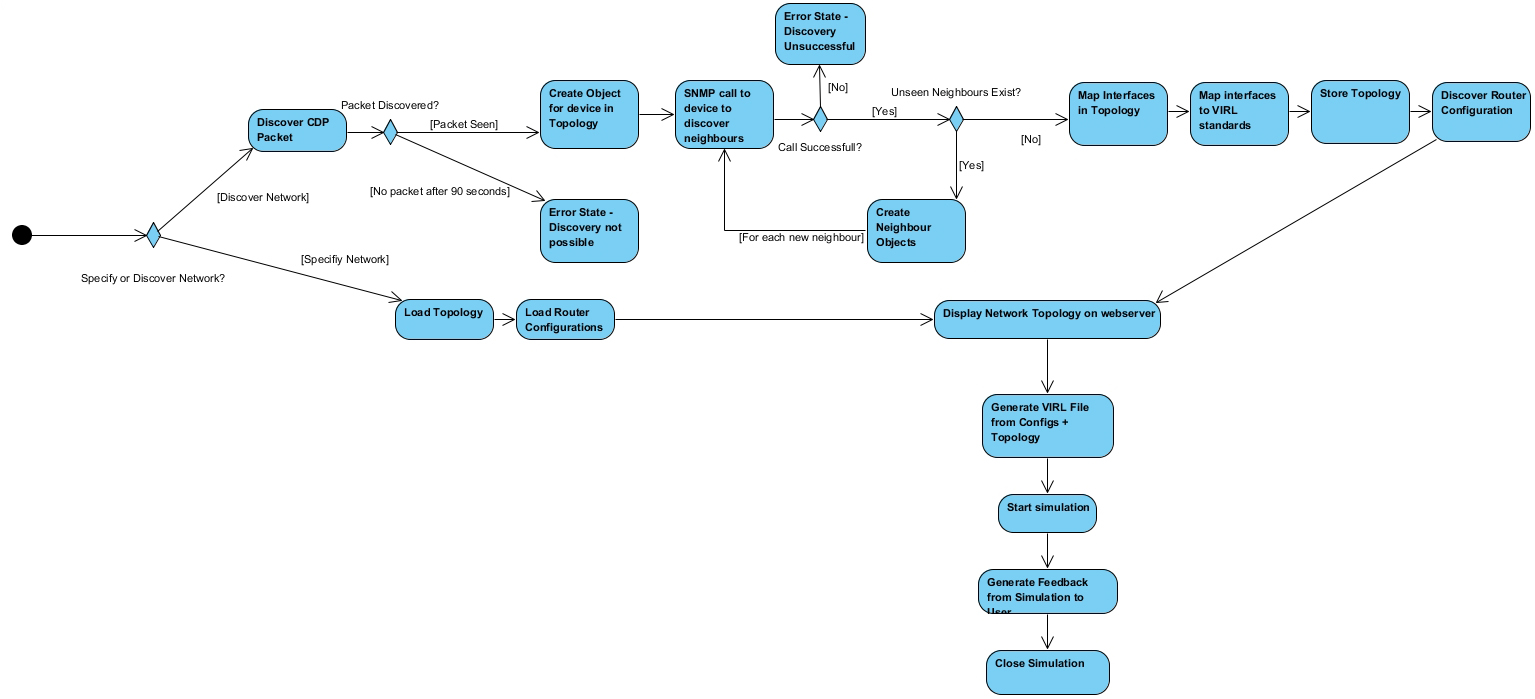
\includegraphics[width=1\textwidth]{activityDiagram.png}
\end{sidewaysfigure}

\section{Network Creation}

An emulated network can be created using two distinct inputs, the first is a copy of the configuration files for all devices in the network which will determine how the components interact with one another. For example, a configuration file can provide the settings for a routing protocol such as OSPF, specifying information required to exchange routes with other devices and choosing the networks they wish to advertise to their peers. The second input is a form of detailing the physical layout of the network, representing the devices as nodes and their inter-device links as edges. Representing this data in a format that is easily readable by a program allows the proposed tool to create emulation with all the interfaces and connections of the physical network, an accurate reproduction of these components ensures that the emulation will behave in the same way as it's physical counterpart.

\textit{Todo: Extracts of Config files and visio/json}

The proposed tool will provide two options for creating an emulated network. First allowing a user to create a version of a well-known network by allowing the input of already existing configuration backups and topology definitions from tools such as Rancid or Opsware. Alternatively, the user will be able to create an emulated version of their local network by using the tool to discover, map and backup their local devices before passing the information on to the simulation element.

\subsection{Explicit Input:}

A well-maintained network will have two components of management, the first is a detailed collection of network diagrams detailing the positions of routers and switches, the interfaces used for these links and any IP addressing these connections have. Tools used for the creation of these documents are programs such as Microsoft Visio or yED, these tools enable a Network Engineer to draw their diagrams and save them in a user-friendly visual format. A further extension of these tools allows the saving of a topology in a programmer-friendly format such as json or xml, the proposed tool will investigate using this data format for representing the emulated network. Once the topology of the network has been created it has no defined behaviour.

The second management process is a backup tool of network device configurations, large enterprise keep a backup of all router configurations as a precaution in case of unintended changes or hardware failure. If given access to these backups the proposed tool will be able to create an emulated network whose behaviour is defined by these files.

\subsection{Network Discovery}

For networks that do not have the management techniques defined above, the tool will also be able to discover devices and create an emulated version dynamically. As before, the network will require both the topology definition and the device configurations to function. In order to gather this information it will utilise some existing network technologies and standards in order to gather the information required in the most efficient method possible.

In order to map the network topology dynamically, the proposed tool will use a combination of SNMP and CDP/LLDP in order to discover the devices in the local network. These technologies, when combined will allow for the tool to create a representation of the network in an edge-and-node format which can be parsed in the emulation software. CDP is a protocol created by Cisco which details a devices local neighbours giving information such as the neighbour's hostname, device type, IP Address, the connections local port and destination port. This information can be gathered from a device by using a standard called SNMP (Simple Network Management Protocol)

Network configuration files can be extracted from running devices in multiple ways, the most common is to log on to a device and copy it's configuration to a network store such as a tftp (Trivial File Transfer Protocol) server where they are stored for later use. An alternative method is through further use of SNMP to poll a device for it's configuration which is returned over a terminal. The tool will use one of these methods to connect to and store a devices configuration. Once both the topology and the configuration of a network is obtained, it can then be passed to Emulation.

\section{Network Representation}

Although the VIRL system provides a topology view for running simulations, I am not intending on using this as part of the proposed tool. Instead, I will investigate methods of displaying a network using the information gathered in the Network Discovery section. I aim to investigate tools such as yED which allows the use of extensions to interact with network drawings. For example, when a topology has been drawn and displayed, it may carry additional attributes such as it's IP Address, using this information the graphing software can be extended to implement features such as a terminal emulator for direct access to a device, or an API for sending defined commands to an emulated network. In addition to the interaction with the emulation, I will also investigate methods of representing feedback from devices. This information can be displayed directly on the visual topology with labels such as the status of a network connection and it's current throughput. This idea can be extended and the use of colour on a network link can show the forwarding path for a destination IP address from it's source. Any changes made to the routing configuration during this time will be reflected by the colour of the links and any impact of the forwarding tables for a destination can be seen.

In addition to the feedback required from a visual representation of a network, there also needs to be a level of interactivity with the network view. A topology can be viewed as it's physical layout but it may have other configurations underneath this layer such as Autonomous Systems, Routing Areas or Redundancy Pairs. This information should be viewable by changing a filter on the network representation as it gives a more granular view on how the network components interact with one another. Adding these extra filters will enable a Network Engineer to view the impact of planned changes on additional aspects of the network which may not have been considered previously.

\section{Network Emulation}

The proposed tool will use Cisco's Virtual Internet Routing Lab (VIRL) as it's platform for simulation, this was chosen as it provides a full Cisco IOSv image for network components which can scale more efficiently that other simulation platforms. In the proposed tool VIRL will be used as a back-end technology and the proposed tool will not make use of the Eclipse-based VM Maestro interface. The User can interact with devices by using SSH to connect to a jumphost which will provide access to the components using the management network which VIRL creates. 

In order to utilise VIRL to its fullest potential the proposed tool will connect to VIRL using it's defined REST API. From initial research it is understood that a simulation can be created by creating a request to the VIRL server and including a defined .virl file. Upon receiving this file the VIRL host will create a simulation based on the on the topology defined in the file. Information about a simulation can also be obtained by making a separate request to the server for a list of running simulations. The proposed tool will make use of both of these features and allow the server to create an emulation, gather information about the emulated network and interact with the network.

\section{Interaction}

The tool will allow a user to interact with their emulated network in a variety of ways. A traditional terminal access will be provided through the web simulation as this is the primary way that an Engineer will interact with and make changes to a real network. In addition to terminal access, the tool will also investigate non-traditional methods of interaction, one benefit of producing a network diagram is the possibility of directly interacting with components in the topology, making changes such as shutting interfaces down or rebooting hardware.

Interaction with network components will provide feedback to the user through the graphical interface provided in the 'Network Representation' section. This section of the tool will display the network dynamically, using information gained from devices such as the forwarding table or bandwidth usage on a link. This information will be interpreted by the graphing software and will provide visual feedback of a network change, such as using coloured links to show a forwarding path through a network.

Connection to the emulation will be provided through a server connected to both a management network within the emulation and a public facing interface for connections from the internet. This server will facilitate the traditional command-line based connections by acting as a jumphost into the network. In addition to command-line access this server will also host a python-based web API which will allow the more unconventional methods of interaction through using networking APIs such as Cisco's OnePK tool set.

\section{Requirements}

\begin{tabular}{|l|p{12cm}|}
	\hline Requirement ID: & 1 \\ 
	\hline Description: & The system must be able to discover a physical network layout \\ 
	\hline Rationale: & A user needs to be able to discover and emulate an undocumented network \\ 
	\hline Type: & Functional \\ 
	\hline Design Constraint: & No \\ 
	\hline Fit Criteria: & A user can create an accurate model of their local network \\ 
	\hline 
\end{tabular}
\newline
\vspace*{0.5 cm}
\newline
\begin{tabular}{|l|p{12cm}|}
	\hline Requirement ID: & 2 \\ 
	\hline Description: & The system must accept existing network information \\ 
	\hline Rationale: & A user needs to be able to create a emulation based on a well-documented network \\ 
	\hline Type: & Functional \\ 
	\hline Design Constraint: & No \\ 
	\hline Fit Criteria: & A user can create an accurate model based on existing network information \\ 
	\hline 
\end{tabular} 
\newline
\vspace*{0.5 cm}
\newline
\begin{tabular}{|l|p{12cm}|}
	\hline Requirement ID: & 3 \\ 
	\hline Description: & The system will discover Cisco Devices \\ 
	\hline Rationale: & The tool needs to discover unknown Cisco devices on a network \\ 
	\hline Type: & Functional \\ 
	\hline Design Constraint: & No \\ 
	\hline Fit Criteria: & All devices on the local topology will be discovered \\ 
	\hline 
\end{tabular}
\newline
\vspace*{0.5 cm}
\newline
\begin{tabular}{|l|p{12cm}|}
	\hline Requirement ID: & 4 \\ 
	\hline Description: & The system will extract configurations from Cisco devices \\ 
	\hline Rationale: & Configuration files are required in order to emulate the behaviour of devices \\ 
	\hline Type: & Functional \\ 
	\hline Design Constraint: & No \\ 
	\hline Fit Criteria: & The configuration of each discovered device is extracted \\ 
	\hline 
\end{tabular}
\newline
\vspace*{0.5 cm}
\newline
\begin{tabular}{|l|p{12cm}|}
	\hline Requirement ID: & 5 \\ 
	\hline Description: & The system will produce a document detailing the physical layout of the network \\ 
	\hline Rationale: & A topology document will allow the tool to visually represent a network \\ 
	\hline Type: & Functional \\ 
	\hline Design Constraint: & No \\ 
	\hline Fit Criteria: & A document is produced which details the topology \\ 
	\hline 
\end{tabular}
\newline
\vspace*{0.5 cm}
\newline
\begin{tabular}{|l|p{12cm}|}
	\hline Requirement ID: & 6 \\ 
	\hline Description: & A topology map must be produced in less than 1 minute \\ 
	\hline Rationale: & Allows the discovery of a network to be efficient so it is of use to a network engineer \\ 
	\hline Type: & Non-functional \\ 
	\hline Design Constraint: & No \\ 
	\hline Fit Criteria: & Device discovery takes one minute or less \\ 
	\hline 
\end{tabular}
\newline
\vspace*{0.5 cm}
\newline
\begin{tabular}{|l|p{12cm}|}
	\hline Requirement ID: & 7 \\ 
	\hline Description: & Router configurations must be extracted in an efficient method \\ 
	\hline Rationale: & Lessens the time taken to produce a working emulation \\ 
	\hline Type: & Non-functional \\ 
	\hline Design Constraint: & No \\ 
	\hline Fit Criteria: & Configuration Extraction takes three minutes or less \\ 
	\hline 
\end{tabular}
\newline
\vspace*{0.5 cm}
\newline
\begin{tabular}{|l|p{12cm}|}
	\hline Requirement ID: & 8 \\ 
	\hline Description: & Connections to Production devices must not compromise security \\ 
	\hline Rationale: & Production devices can be left vulnerable if security is lessened \\ 
	\hline Type: & Non-functional \\ 
	\hline Design Constraint: & Yes \\ 
	\hline Fit Criteria: & The tool requires no additional access to systems when compared to an industry standard tool \\ 
	\hline 
\end{tabular}
\newline
\vspace*{0.5 cm}
\newline
\begin{tabular}{|l|p{12cm}|}
	\hline Requirement ID: & 9 \\ 
	\hline Description: & Any Cisco device can be represented within a emulation \\ 
	\hline Rationale: & A device must be able to be represented in an emulation regardless of model \\ 
	\hline Type: & Functional \\ 
	\hline Design Constraint: & No \\ 
	\hline Fit Criteria: & Any standard Cisco router will be represented in an emulation \\ 
	\hline 
\end{tabular}
\newline
\vspace*{0.5 cm}
\newline
\begin{tabular}{|l|p{12cm}|}
	\hline Requirement ID: & 10 \\ 
	\hline Description: & Network Discover will be able to cope with non-router devices \\ 
	\hline Rationale: & Not every network will be a collection solely of interconnected routers \\ 
	\hline Type: & Functional \\ 
	\hline Design Constraint: & No \\ 
	\hline Fit Criteria: & The discover will cope with Layer-2 devices such as switches and will deal with them effectively \\ 
	\hline 
\end{tabular}
\newline
\vspace*{0.5 cm}
\newline
\begin{tabular}{|l|p{12cm}|}
	\hline Requirement ID: & 11 \\ 
	\hline Description: & All interface types will be represented in an emulation \\ 
	\hline Rationale: & Cisco devices have multiple types of interfaces that need to be included \\ 
	\hline Type: & Functional \\ 
	\hline Design Constraint: & No \\ 
	\hline Fit Criteria: & Any standard Cisco interface will be represented in a emulation \\ 
	\hline 
\end{tabular}
\newline
\vspace*{0.5 cm}
\newline
\begin{tabular}{|l|p{12cm}|}
	\hline Requirement ID: & 12 \\ 
	\hline Description: & Physical interfaces will be converted into an equivalent weighting in the emulation \\ 
	\hline Rationale: & Different interface types will have different characteristics which will influence routing \\ 
	\hline Type: & Functional \\ 
	\hline Design Constraint: & No \\ 
	\hline Fit Criteria: & An interface will influence routing in the same way both in real hardware and in a emulation \\ 
	\hline 
\end{tabular}
\newline
\vspace*{0.5 cm}
\newline
\begin{tabular}{|l|p{12cm}|}
	\hline Requirement ID: & 13 \\ 
	\hline Description: & Configurations will be converted into an equivalent emulation configuration \\ 
	\hline Rationale: & The emulation must include exactly the same features and characteristics in order to be of use as a testing platform \\ 
	\hline Type: & Functional \\ 
	\hline Design Constraint: & No \\ 
	\hline Fit Criteria: & There will be no configuration loss in the emulation when compared to the real hardware \\ 
	\hline 
\end{tabular}
\newline
\vspace*{0.5 cm}
\newline
\begin{tabular}{|l|p{12cm}|}
	\hline Requirement ID: & 14 \\ 
	\hline Description: & The tool will produce a Cisco VIRL file  \\ 
	\hline Rationale: & The emulation engine, Cisco VIRL represents a topology in a VIRL file \\ 
	\hline Type: & Functional \\ 
	\hline Design Constraint: & No \\ 
	\hline Fit Criteria: & A VIRL file defining the topology is produced \\ 
	\hline 
\end{tabular}
\newline
\vspace*{0.5 cm}
\newline
\begin{tabular}{|l|p{12cm}|}
	\hline Requirement ID: & 15 \\ 
	\hline Description: & The produced emulation file will be a valid VIRL configuration file  \\ 
	\hline Rationale: & The produced file will be passed to an external process for emulation and therefore must be complete and valid \\ 
	\hline Type: & Non-Functional \\ 
	\hline Design Constraint: & Yes \\ 
	\hline Fit Criteria: & All produced VIRL files will be accepted as valid by the VIRL engine \\ 
	\hline 
\end{tabular}
\newline
\vspace*{0.5 cm}
\newline
\begin{tabular}{|l|p{12cm}|}
	\hline Requirement ID: & 16 \\ 
	\hline Description: & The tool will automatically produce a simulation when a valid VIRL file is created  \\ 
	\hline Rationale: & An emulation needs to be produced without any input by the user or any third-part GUI \\ 
	\hline Type: & Functional \\ 
	\hline Design Constraint: & No \\ 
	\hline Fit Criteria: & An emulation is created as part of the tool running  \\ 
	\hline 
\end{tabular}
\newline
\vspace*{0.5 cm}
\newline
\begin{tabular}{|l|p{12cm}|}
	\hline Requirement ID: & 17 \\ 
	\hline Description: & The emulated network will be accessible through the internet  \\ 
	\hline Rationale: & The emulation needs a method of access to the network \\ 
	\hline Type: & Functional \\ 
	\hline Design Constraint: & No \\ 
	\hline Fit Criteria: & The emulation is available online  \\ 
	\hline 
\end{tabular}
\newline
\vspace*{0.5 cm}
\newline
\begin{tabular}{|l|p{12cm}|}
	\hline Requirement ID: & 18 \\ 
	\hline Description: & The tool will provide a single server as a point of entry to the emulation  \\ 
	\hline Rationale: & Having multiple publicly available devices on the internet poses a security risk \\ 
	\hline Type: & Functional \\ 
	\hline Design Constraint: & No \\ 
	\hline Fit Criteria: & The tool provides one single publicly routable ip address for access  \\ 
	\hline 
\end{tabular}
\newline
\vspace*{0.5 cm}
\newline
\begin{tabular}{|l|p{12cm}|}
	\hline Requirement ID: & 19 \\ 
	\hline Description: & The user will be able to view a diagram of the discovered network before emulation  \\ 
	\hline Rationale: & A user will want to check the discovered network is correct before creating an emulation \\ 
	\hline Type: & Functional \\ 
	\hline Design Constraint: & No \\ 
	\hline Fit Criteria: & A diagram is produced before the network is emulated  \\ 
	\hline 
\end{tabular}
\newline
\vspace*{0.5 cm}
\newline
\begin{tabular}{|l|p{12cm}|}
	\hline Requirement ID: & 20 \\ 
	\hline Description: & The emulated network will contain a separate management network for the external server to communicate on \\ 
	\hline Rationale: & A management network will ensure that any management tools will not interfere with the emulation routing \\ 
	\hline Type: & Functional \\ 
	\hline Design Constraint: & No \\ 
	\hline Fit Criteria: & The management of the network is on an entirely separate network to the emulation  \\ 
	\hline 
\end{tabular}
\newline
\vspace*{0.5 cm}
\newline
\begin{tabular}{|l|p{12cm}|}
	\hline Requirement ID: & 21 \\ 
	\hline Description: & The user will be able to interact with an emulation in a conventional way \\ 
	\hline Rationale: & A user will want to interact with the emulation in a familiar way \\ 
	\hline Type: & Functional \\ 
	\hline Design Constraint: & No \\ 
	\hline Fit Criteria: & The user will have command-line access to any router produced in the emulation  \\ 
	\hline 
\end{tabular}
\newline
\vspace*{0.5 cm}
\newline
\begin{tabular}{|l|p{12cm}|}
	\hline Requirement ID: & 22 \\ 
	\hline Description: & The user will be able to influence the network in non conventional ways \\ 
	\hline Rationale: & The tool will provide other methods of influencing the emulated network \\ 
	\hline Type: & Functional \\ 
	\hline Design Constraint: & No \\ 
	\hline Fit Criteria: & The user will influence the network in methods other than CLI  \\ 
	\hline 
\end{tabular}
\newline
\vspace*{0.5 cm}
\newline
\begin{tabular}{|l|p{12cm}|}
	\hline Requirement ID: & 23 \\ 
	\hline Description: & The network diagram will produce visual feedback representing the current state of the network \\ 
	\hline Rationale: & The user will want to see methods other than the CLI for understanding the behaviour of the network \\ 
	\hline Type: & Functional \\ 
	\hline Design Constraint: & No \\ 
	\hline Fit Criteria: & Visual feedback is produced on the CLI  \\ 
	\hline 
\end{tabular}
\newline
\vspace*{0.5 cm}
\newline

\section{Risks}

The project has the following risks identified which could impact development:

\begin{itemize}
  \item{Constraints on access to University infrastructure}
  \begin{itemize}
    \item{External to the VIRL Server there may be a requirement to have an external server which is able to access the VIRL network - as this is in the domain of IT Services, this may not be possible}
  \end{itemize}
  \item{VIRL may not provide the functionality this project requires}
  \begin{itemize}
    \item{As the current implementation of the Cisco VIRL service is pre-release, there is some aspect of missing functionality or suffers from pre-release bugs}
  \end{itemize}
  \item{Added complexity through lack of documentation}
  \begin{itemize}
    \item{As Cisco VIRL is still pre-release and limited availability there is a lack of documentation and community support for the product}
  \end{itemize}
  \item{Requirement of Python in Cisco Development}
  \begin{itemize}
    \item{Cisco products (In particular onePK) require a knowledge of Python. This is a new language that is not well known to the developer. Therefore there may be added difficulty in understanding its function.}
  \end{itemize}
  \item{Risk of hardware failure}
  \begin{itemize}
    \item{Project may be delayed in the event of hardware failure, particularly the VIRL Server in place which requires a significant time investment to install}
  \end{itemize}
\end{itemize}

\section{Equipment Used}


\subsection{Servers}

For the production of this tool it is understood that two distinct servers are required, one local server which can handle the Network Discovery aspect of the tool and a secondary server which is contained within the VIRL emulation which will handle feedback based on changes to the emulated network. These two servers will be in contact with one-another throughout the course of a tools use. There are two solutions available for these servers, the first being a standard Linux server distribution and the second being a Windows Server installation.

One requirement of the proposed tool is the ability to display a network topology for the user to understand the layout of an emulated network. This will take form in a web browser, therefore there needs to be some aspect of a GUI on the server itself. Because of this, a standard Linux server CLI has been ruled out in favour of a more desktop-like server experience.

A second requirement of the proposed tool is the ability to interact with protocols such as CDP and SNMP. From initial research this level of interaction with packet-level networking is considerably easier and more flexible on a Unix-based operating system as existing tools can be run in a standard shell to interact with CDP. In addition to this, there are additional python libraries which can create and/or intercept packets which require a Unix operating system to run.

Due to the two requirements outlined above, it is proposed that a Linux desktop or server with display server should be used for this work. In particular, Ubuntu will be used for it's user-friendliness in comparison to other distributions.

\subsection{Networking Equipment}

The proposed tool is intended to be deployed in a real-world environment, however due to the constraints I have on physical equipment for this project I have opted to create this topology in GNS3 (See ‘Existing Solutions’). GNS3 provides full simulation of IOS images and therefore is the closest representation of physical equipment. These simulations were created and run on a Windows PC using the GNS3 client. In addition to router simulation, GNS3 also has support for Virtualbox integration within the tool, this allows Virtual Servers to be connected to a topology and function correctly on a network. I will use this functionality in order to connect the Network Discovery server (as discussed in the previous section) to a separate emulated network. The use of GNS3 rather than real equipment enables a more efficient development process as work does not need to be done on-site with the physical equipment. In addition to this, the use of an emulated network allows a more thorough testing process as a multitude of testing scenarios can be created quickly, enabling more in-depth test procedures.

\subsection{Python}

In addition to physical equipment, the tool will also use Python as it's primary language. This has been selected due to it's flexibility and existing position in the networking development world. Due to this foothold Python has an extensive set of libraries which facilitate easier access and processing of network information.

From initial research, Python can be used to create REST network connections which allow it to interface directly with VIRL to create, edit and destroy existing simulations. Selecting Python will enable the tool to seamlessly discover networks, collate network information, create a simulation and interact with a simulation.

\subsection{CDP - Cisco Discovery Protocol}

A second software that has been identified is CDP, a proprietary protocol created by Cisco which facilitates mapping of a network through local neighbour advertisements. This protocol is enabled on all Cisco devices by default, sending an advertisement to all local neighbours every 60 seconds. In this advertisement the device specifies it's hostname, whether the device is a router or a switch, the model number of the device and the interface on it's local side on which it is sending the advertisement. 

From an advertisement the receiving device can piece together all the received information in order to build a picture of it's local network. An example of a CDP table for a device is shown below. From this table it can be seen that there are two local routers (R2 and R3) on the local interface FastEthernet0/0. In addition to this information, it can also be seen that R2 and R3 can see R1 on their FastEthernet0/0 interfaces, with further analysis, because R1 can see R2 and R3 on the same local interface it can be inferred that there is a switch connecting all three devices.

\begin{lstlisting}
R1# show cdp neighbors
Capability Codes: R - Router, T - Trans Bridge, B - Source Route Bridge
S - Switch, H - Host, I - IGMP, r - Repeater

Device ID        Local Intrfce     Holdtme    Capability  Platform  Port ID
R2               Fas 0/0            157         R S I     3725      Fas 0/0
R3               Fas 0/0            156         R S I     3725      Fas 0/0
\end{lstlisting}

\subsection{SNMP - Simple Network Management Protocol}

An additional tool that will be used is SNMP, Simple Network Management Protocol \citep{case1989simple} is a protocol designed to allow access to sensors on a networked device. The protocol relies on a Management Information Base (MIB) which defined on a Vendor basis. Inside these MIBs there are defined Object Identifiers (OIDs) which relate to a specific sensor on the device. Access to this OIDs are managed on the device, requiring a community string which a plaintext password in SNMPv2 as a security device to prevent unauthorised access. Additional security is provided by only allowing Read-only access to OIDs which prevent malicious attacks to a system. For the purpose of this project there will only ever be a need for Read-only access, this is due to the fact that Read-Write is disabled on devices due to security concerns.

When making a call to an SNMP Agent, specifying the OID and community string the device returns a plaintext response with the requested information. This can be parsed for and adapted for use in the Network Discovery portion, or alternatively can be used in the Network Feedback sections in order to understand forwarding information. The following output shows the returned information for a call to OID `.1.3.6.1.2.1.2.2.1.2', the OID which holds information relating to the interfaces on a device.

\begin{lstlisting}
rob@netman-server:~$ snmpwalk -v 2c -c public 172.30.0.1 .1.3.6.1.2.1.2.2.1.2
IF-MIB::ifDescr.1 = STRING: FastEthernet0/0
IF-MIB::ifDescr.2 = STRING: Serial0/0
IF-MIB::ifDescr.3 = STRING: FastEthernet0/1
IF-MIB::ifDescr.4 = STRING: Serial0/1
IF-MIB::ifDescr.5 = STRING: Serial0/2
IF-MIB::ifDescr.6 = STRING: Serial0/3
IF-MIB::ifDescr.8 = STRING: Null0
IF-MIB::ifDescr.13 = STRING: Loopback0
IF-MIB::ifDescr.14 = STRING: NVI0
\end{lstlisting}

\subsection{SDN Sources using OnePK}

OnePK is Cisco's current offering on the Software Defined Networking marketplace and allows a programmatic approach to controlling and extracting information from Cisco devices.

Software Defined Networking (SDN) is a relatively new concept in the network space and although has not fully been adopted in real-world standards it can be used to extract information from routers with a relatively small footprint in production. Where traditionally a routing table of a Router would be extracted by using a tool such as a screen-scraper or SNMP, the routing table from a OnePK enable device can be requested using an API-like interface. This approach scales more efficiently than using CLI-scraping as the data can be requested through an constant connection rather than opening a telnet/SSH session. Data returned from a OnePK call can either return data in a structured format or as a copy of the text displayed on the CLI. In the case of the structured data the appropriate information can be accessed directly, in the case of screen data it can be extracted using regular expressions.

With regards to this project, OnePK will be used in the Network Feedback section in order to process information such as forwarding tables. In addition to this, it can also be used to control the network as a whole, allowing the tool to make changes to interface states or costs in order to influence routing decisions.

\chapter{Implementation}

\section{Router Discovery:}

\begin{center}
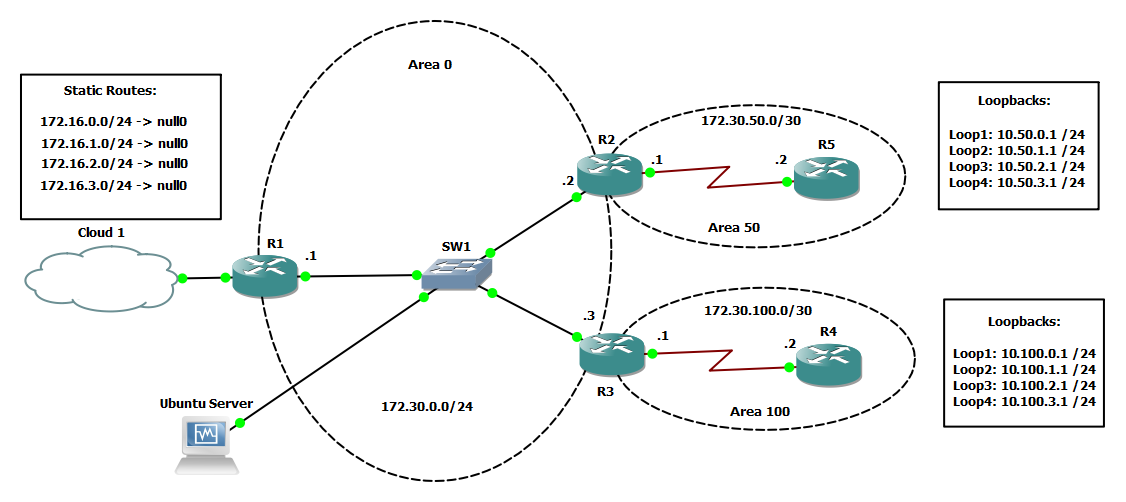
\includegraphics[width=0.8\textwidth]{Lab-Design.png}
\end{center}

A key feature of the simulation tool is the ability to replicate a 'Real-world' network in emulated space. In order to gather the information required for this feature an extra tool set for Network Discovery has been created. This allows a user to discover devices on the network and extract interface information and router configurations in order to build an emulated instance of the network.

For the development of this Router Discovery tool the above topology was created and used. As explained earlier this is implemented within GNS3 to utilise it's simulation of real IOS images. The above shows a Topology I have created as a use-case for simulation testing, however in order to add the Network Discovery tool I have included an Ubuntu 14.04 server and a connection to the Internet (Cloud 1).

The Ubuntu server is implemented using VirtualBox integration within GNS3 and allows direct connection to the 172.30.0.0/24 network. This Ubuntu server will hold the tool used for Router Discovery and Configuration Extraction. As this server is sitting on the same private network as all of the routers this allows me to find all the routers using defined ip addresses or through using CDP.

The connection to the Internet is provided through the cloud in the diagram above. This is inbuilt functionality within GNS3 which allows the topology to interface with the local host’s connection. This is implemented by adding a loopback to the local PC and bridging the internet connection to this loopback. GNS3 then connects to this loopback address and provides an interface to the Internet in the form of the Cloud object. Once this connectivity is provided the topology has a defined router which is used for internet connections, in this scenario R1 provides the connection. This router is then configured to provide dhcp to any servers on the local subnet, providing a default gateway and DNS Servers for the connected hosts. This router is also configured to provide NAT services in order to allow these private addresses to communicate to the outside world. Once internet connectivity is established the system can deploy.

Data from these devices will be extracted using an SNMP agent. Cisco Discovery Protocol (CDP) is a protocol created to collate important information about a Cisco device and broadcast it out to the network. For example the {\tt show cdp neighbours} command on R1 above yields the following information:



From the above I can see that R1 is directly connected to two routers, R2 and R3. I can also see which interface each side of the connection is on. As both are currently sitting on {\tt Fas 0/0} this indicates that they are both connected to a switch. This is valuable information when understanding the topology as it defines which cables are connected where.

This information is useful as it allows a user to view what devices are directly connected without having access to an overall topology. However, the need for physically connecting to the device and running commands on the CLI is  not optimal for an automated system as is the one being created. In addition to the process of logging on to a router, there is also the credentials required to facilitate this access. This may be an extra method of access that a Network Administrator would not be comfortable giving to an automated system. As a resolution to these issues the tool will utilise SNMP as a way of polling devices, in particular a Cisco MIB called CISCO-CDP-MIB allows this information to be gathered and accessed using SNMP. From this MIB I can gather the hostname and ip address of each neighbour to a device and from this I can then poll the neighbour to find details of his neighbour. This can be done programmatically until no further neighbours are found.

Once all the required routers are discovered the tool will then begin to implement extraction of each router's configurations. It will do this by using SSH to connect to each Router that has been identified and back-up it's starting configuration to the server. The server will then have knowledge of the network topology from the SNMP data and a copy of each Router configuration. From here a valid .virl file can be created of the topology. 

\section{VIRL File Creation}

The VIRL engine expects a defined file type which is used to define the topology layout and the configurations used on first run of the simulation. In order to have the real-world network elements correctly represented in the simulation the topology and network configurations need to be correctly reflected in the VIRL file. 

In order to convert the extracted data into the VIRL file I have created a python program on the local server. This program will parse each router in the topology and it's accompanying configuration file and create a correct virl file. Once this parsing is complete the topology is ready for simulation.

\section{Simulation}

Once a correct .virl file has been created the tool is ready to begin the simulation. This can be done in one of two ways, either by opening the VM Maestro client and loading the simulation manually...

\textit{Note: The available simulation methods supported within VIRL are currently not understood. It is clear that the simulation can be started using the GUI with a correct virl file, however this would not work well with the tool design as it requires the use of another program. The desired method would be to use a command line interface to to create a simulation. Details of that simulation can then be gathered using the REST API on the VIRL server.}

Simulations within VIRL will be created using a setting on the simulation engine known as a 'Private Simulation Network'. This option creates a management network on the simulation which allows access to the management ports of the Routers on the topology. In addition to this it also provides a Linux container (LXC) on the network on this management network. One issue that arises from keeping this tool separate from VM Maestro is that the ip addressing schema produced by VIRL for these hosts is only viewable from the GUI. I have identified that this information is available be sending an authenticated REST request to the API running on the VIRL server, the response to this will provide information regarding the simulation details. A particular detail of note is information relating to this LXC host is it's ip address (Which is defined by VIRL and is allocated per simulation) or a unique port number to connect on via the VIRL server ip. This allows access from outside of the VIRL simulation. The below output from an API call details this information:

\begin{lstlisting}

"rob.My_Topologies@topology-gymofc.virl.~lxc-flat.External Address": {
    "Annotation": "131.231.97.151",
    "SimulationHost": "158.125.102.75",
    "managementIP": "131.231.97.151",
    "simExpires": null,
    "simID": "My_Topologies@topology-gymofc",
    "simLaunch": "2015-01-06T16:06:59.534563",
    "simStatus": "ACTIVE"
  },
  "rob.My_Topologies@topology-gymofc.virl.~lxc-flat.External Port": {
    "Annotation": "59313",
    "SimulationHost": "158.125.102.75",
    "managementIP": "59313",
    "simExpires": null,
    "simID": "My_Topologies@topology-gymofc",
    "simLaunch": "2015-01-06T16:06:59.534563",
    "simStatus": "ACTIVE"
  },

\end{lstlisting}

The above can provide flexibility to the way the system connects to VIRL. There are two methods of connection using the LXC host, the first is to use the ip address assigned to the host, this information is provided in the "External Address" section. However this address can be dynamically assigned by the VIRL server and could be any address on the 131.231.97.128/25 network. A second method is to use the "External Port" section above, instead of using the ip address assigned to the LXC host this instead uses the primary ip address of the VIRL server (158.125.102.75). The creation of the simulation informs the server to begin listening on this port, any connections to the server on this port will automatically be passed through to the LXC host. Due to this, I have opted to add a call to the API in order to check which ip address has been assigned. If this were not the case then only one simulation could be made at any given time, this would be achieved by defining which port was used for access through the VIRL Server ip.

\section{Network Monitoring}

\textit{To do: Investigate whether current Open Source solutions such as Cacti or MRTG will provide the output require or whether a new solution would be added as part of this project}

\subsection{SNMP Monitoring}

IOSv instances, the focus of this tool support SNMP just as a physical router would. Using this access I can set up an SNMP Monitor on a server within the simulation which could provide detailed statistics such as interface counters. Using this information the system can determine at a high-level where traffic is flowing.

\subsection{Netflow}

Cisco Flexible Netflow is supported by Cisco IOSv and gives a more detailed view of traffic across router interfaces. Configuring each IOSv instance as a Flow Exporter and adding an collector such as Cacti will provide a detailed breakdown of traffic based on it's Layer 3 and 4 information. This adds further granularity to the testing evidence that is created.

\subsection{Packet Capture}

All interfaces within VIRL have a defined 'tap' interface on the VIRL Server, this can be used for packet captures. Using a packet capture in addition to the Netflow and SNMP will allow the tool to inspect the traffic at a much more granular level. One use case of this would be the testing of a routing change on an established session and how an application can deal with this.

\textit{Note: Access to these tap interfaces may require access to the VIRL server in the admin role}
 

\section{Testing Scenarios}

To support the development of this project I have created a set of network topologies with complex configurations. These are a representation of a network which a user may wish to simulate and can demonstrate added complexities which may be encountered in a real-world networks. In addition to this, they provide an already established routing platform which can be used for testing network changes. As described in the previous section "Equipment Used" these topologies have been created inside of GNS3.

\subsection{Topology 1: Multi-area OSPF}

\begin{center}
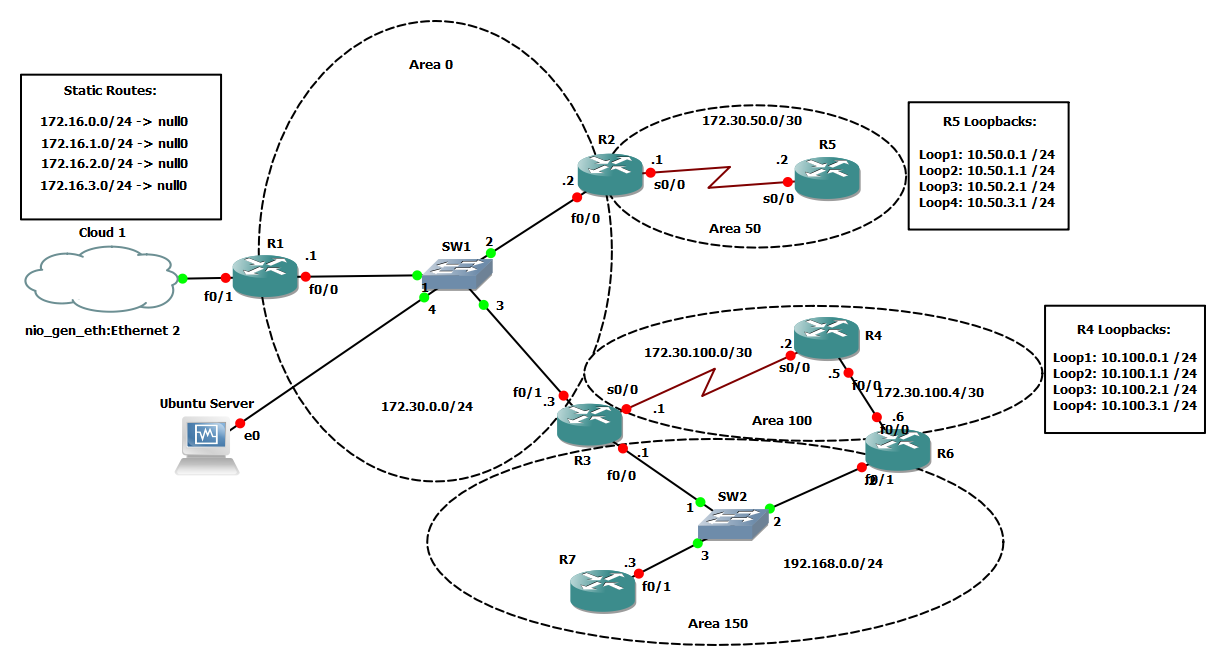
\includegraphics[width=0.8\textwidth]{OSPF-Topology.png}
\end{center}

I have designed this Topology to represent a simple network with a complex OSPF routing set-up, which may be a possible scenario that a network engineer may wish to experiment with before implementing changes in Production.

The topology represents the OSPF backbone of a large enterprise network, it includes three OSPF areas; area 0 (Backbone), area 50 and area 100. In this scenario R2 and R3 are taking the role of Area Border Routers (ABR) and providing route summarisation between the areas. For both area 50 and area 100 there are also addition Loopbacks created on the end routers which provide additional routes for this summary.

In addition to the routes being introduced via the loopbacks on R4 and R5 the topology also injects external routes into OSPF on R1. These are static routes defined on R1 which represent routes from either the Internet or routes from another routing protocol such as EIGRP, IS-IS or BGP. In this form the routes are sent to null 0 (blackhole) as there is no need for connectivity to them.

\subsection{Topology 2: EIGRP Based Routing}

\subsection{Topology 3: Service Provider BGP Topology}

\chapter*{Implementation Notes}

\section*{Simulation Tools}

\subsection*{Simulation Start}

A simulation can be started on the VIRL host itself by specifying the .virl file to be processed and the user workspace for it to be used in. This process is shown below:

\begin{lstlisting}
virl_std_client simengine-launch --virl-file /path/to/starter.virl
Session ID is starter-Ewn0Mn
export STD_SESSION=starter-Ewn0Mn
\end{lstlisting}

\subsection*{REST API}

Details of the current running simulations for an account can be determined via the following URL: http://virl.lboro.ac.uk:19399/roster/rest/

The output of this called is shown in section 4.3

By analysing the output of this data the public ip address of the LXC Host can be determined and access to the simulation can be granted.

\subsection*{LXC Host}

The LXC host is created when the simulation is first started, by selecting the Management Network type as a 'Private Simulation Network'. Upon the start of a simulation an additional Linux Container (LXC) will be created. This container will be available on a public ip address and can be accessed externally (within the Loughborough network)through SSH. Once connected to the container all other hosts on the network are directly connected and can be accessed using their management ip address.

\section*{Connectivity Tools}

\section*{Creation of SNAT Connection}

As described in the LXC Host section, all hosts can be accessed externally by using the LXC host as a jumphost into the simulation. However, this does not provide routing to the outside world. A use-case for the SNAT object would be a single point of exit to the outside world, as would be used in a standard network infrastructure. Connecting a SNAT object to a designated 'external' router can provide access to the entire simulation if required.

\subsection*{Default Routes}

For any devices that require a SNAT object, a route needs to be added on the router for connection to the SNAT object. This can take the form of a default route (below)

\begin{lstlisting}
ip route 0.0.0.0 0.0.0.0 10.254.0.1
\end{lstlisting}

\subsection*{Server IP Addressing}

When connected to a multipoint connection a server is assigned an ip address in the subnet range, this is usually done sequentially. Alternatively this can be defined in the .virl file.

\subsection*{Server DNS}

DNS Servers can be added to a host by editing the /etc/resolv.conf file. Alternatively they can be provided to a server if DHCP is enabled on the router.

\section*{RANCID Installation \& Use}

Look to set up SSH rather than telnet (For security)
\\
Change Protocol type on router side (2vs1)
\\
NOTE: Hostnames in the .cloginrc file need to be lowercase

\section*{Initial Discovery}

Use cdpr on the discovery server in order to discover the default gateway address + port

sudo apt-get install cdpr

sudo cdpr

\section*{Python Path}

 export PYTHONPATH=/opt/cisco/onep/lib/python2.7/site-packages
 
\section*{SNMP to get CDP Neighbors}

snmpwalk -v 2c -c public 172.30.0.1 .1.3.6.1.4.1.9.9.23.1.2.1.1.6.1.2

.1.3.6.1.4.1.9.9.23.1.2.1.1 - Gives information of sh cdp neigh

1.3.6.1.4.1.9.9.23.1.2.1.1.6  - Gives the hostnames of CDP neighbours 

.1.3.1.4.1.9.9.23.1.2.1.1.4 - Gets the ips for the above

.1.3.6.1.4.1.9.9.23.1.2.1.1.7 - Gives local interfaces

.1.3.6.1.2.1.4.1 - Gives ip forwarding (1 is router, 0 is a switch)

.1.3.6.1.4.1.9.9.23.1.2.1.1.7 - Gives interfaces on neighbour

\section{Virl Server Setup}
route add default gw 192.168.1.254 eth0

\section{Change server interface ip}
ifconfig eth1 up 10.254.0.36 netmask 255.255.255.0

\bibliographystyle{plainnat}
\bibliography{bibliography}

\end{document}

